\newpage
\subsection{Caso d'uso UC14: Login con Facebook}
\label{UC14}
\begin{figure}[ht]
	\centering
	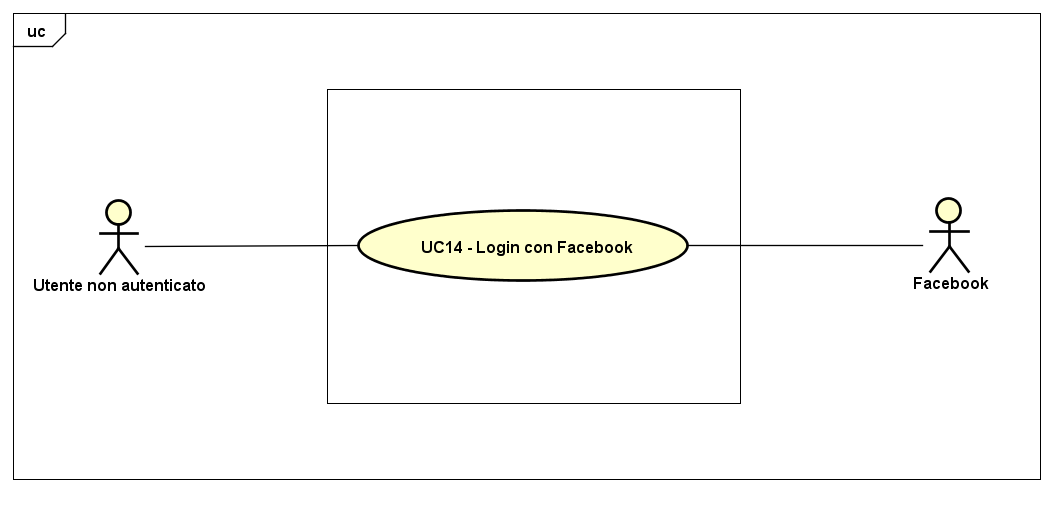
\includegraphics[scale=0.48]{UML/UC14.png}
	\caption{UC14: Login da Facebook}
\end{figure}
\FloatBarrier
\begin{itemize}
	\item \textbf{Attori}: utente non autenticato, Facebook;
	\item \textbf{Descrizione}: l'attore può autenticarsi utilizzando Facebook;
	\item \textbf{Precondizione}: l'attore visualizza la pagina di login e sceglie il login con Facebook;
	\item \textbf{Postcondizione}: l'attore è autenticato;
	\item \textbf{Scenario principale}: l'attore effettua il login tramite Facebook.
\end{itemize}
